
\begin{figure}
    \centering
    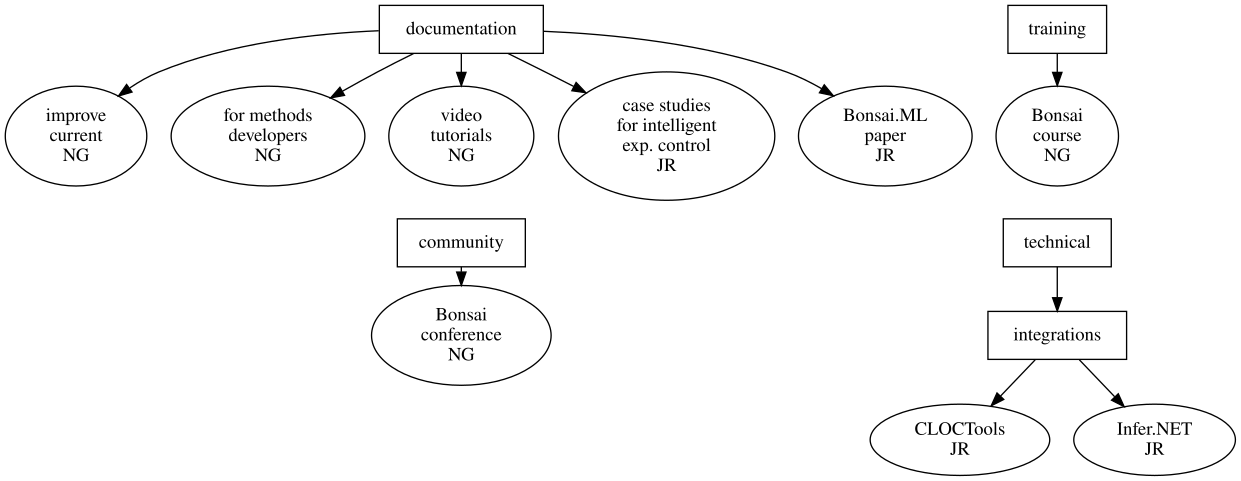
\includegraphics[width=6in]{activitiesGraphs/activities_larger.png}

    \caption{Proposed activities. The initials below each task name indicate
    the responsible team member (JR: Joaquin Rapela, NG: NeuroGEARS Ltd). See
    text for details.}

\end{figure}

\subsection{Approach}

\subsubsection{Aim 1: Documentation}

\paragraph{Background:} The Bonsai.ML project has maintained a strong
commitment to producing high-quality documentation to support both experimental
neuroscience users and machine learning method developers. The current
documentation includes introductory articles with installation guides for each
package, an automatically generated API reference for the C\# codebase, and
illustrative examples demonstrating a range of use cases. However, it lacks
essential statistical explanations of the integrated methods and clear
connections between them, which are critical for non-specialist users to
understand how and when to apply each technique. As a model for improvement, we
look to \href{https://scikit-learn.org/}{scikit-learn}, whose documentation
successfully combines intuitive statistical background, practical tutorials,
and comprehensive API references, and has been key to its widespread adoption.


Our team has been approached by several users of the package who have expressed
concerns about the current state of the documentation, particularly regarding
the documentation structure.  There is redundancy in some places of the
documentation and a lack of clarity in others.
%
These problems make it difficult for users to find the information they need,
leading to unnecessary user-friction driving new users away from the project.

Furthermore, the current documentation does not adequately address the needs of
machine learning method developers. Our team has documented several approaches
for integrating machine learning models into Bonsai, but this information is
currently distributed across various sources, including GitHub repos,
discussion issues, pull requests, and examples. Our project lacks a dedicated,
centralized resource that provides comprehensive documentation for method
developers looking to integrate new machine learning functionality into Bonsai
using the approaches our team has developed.

To address these issues, we have identified several key areas of improvement
that we believe will enhance the usability and accessibility of the
documentation for both experimental neuroscientists and machine learning
methods developers. These include the following tasks.

\paragraph{Tasks:}\mbox{}\\

\begin{description}

    \item[doc\_sickit-learn] Restructure and expand the existing documentation
        to match the \texttt{scikit-learn} documentation style. (4 weeks)

    \item[doc\_examples:] Develop at least 3 new examples demonstrating
        applications of Bonsai.ML to neuroscience problems. These examples will
        cover: real-time visualizations of neural latents, forecasting
        positions and head orientations of mice in augmented reality
        environments, and close-loop control of simulated neural populations.
        Each example will have detailed workflow
        descriptions, information on the models and assumptions, and
        explanations of the datasets. (3 weeks)

    \item[doc\_trouble:] Create a troubleshooting section to address
        common issues users may encounter when using Bonsai.ML packages. This
        section will include solutions to frequently asked questions, common
        errors, and tips for debugging. (2 weeks)

    \item[doc\_videos:] Produce at least 3 video tutorials and demos, hosted on
        YouTube, and embed them directly into the documentation. These videos
        will cover key topics such as installation, user guides, and examples.
        The 3 videos will be: 1) Installation and getting started with
        Bonsai.ML, 2) Integrating custom models into Bonsai using Python, and
        3) Building a Bonsai.ML application to perform closed-loop control of
        neural activity. Video engagement will be monitored by tracking views,
        likes, and comments. (3 weeks)

    \item[doc\_case\_studies:] Create two case studies on intelligent
        experimental control in Bonsai, similar to the
        \href{https://mark-kramer.github.io/Case-Studies-Python/intro.html}{case
        studies for neural data analysis in Python}, or those for
        \href{https://mbmlbook.com/index.html}{model based machine learning},
        by our Microsoft collaborators. Case study one will cover inference
        of mouse kinematics using linear dynamical systems and case study two
        will elaborate on real-time inference and visualisation of neural
        latents. (4 weeks)

\end{description}

\paragraph{Milestones and Indicators:}\mbox{}\\

\begin{description}

    \item[doc\_m1]: Documentation restructured using the \texttt{scikit-learn}
        documentation style.

    \item[doc\_i1]: Documentation updated in the
        \href{https://bonsai-rx.org/machinelearning/}{Bonsai.ML documentation site}.

    \item[doc\_m2]: Dissemination of three new examples of the application of Bonsai.ML to
        neuroscience problems.

    \item[doc\_i2]: Three new examples of the application of Bonsai.ML
        to neuroscience problems published in the
        \href{https://bonsai-rx.org/machinelearning/}{Bonsai.ML documentation site}.

    \item[doc\_m3]: New troubleshooting sections published.

    \item[doc\_i3]: Troubleshooting section including at least 10 common
        issues/error added to the
        \href{https://bonsai-rx.org/machinelearning/}{Bonsai.ML documentation site}.

    \item[doc\_m4]: Three video tutorials produced, uploaded to YouTube, and
        embedded in the documentation.

    \item[doc\_i4]: Three video tutorials published in the Bonsai.ML YouTube
        channel and linked in the
        \href{https://bonsai-rx.org/machinelearning/}{Bonsai.ML documentation site}.

    \item[doc\_m5]: Two case studies on intelligent experimental control
        created.

    \item[doc\_i5]: Two case studies published in a new Case Studies section of
        the
        \href{https://bonsai-rx.org/machinelearning/}{Bonsai.ML documentation site}.

\end{description}

\paragraph{Impact:} Improving the documentation of Bonsai.ML will directly
improve the code's maintainability, reduce technical debt for maintainers and
contributors, and expand the project's reach. The expansion of the
documentation will also greatly enhance usability of Bonsai.ML for two core
communities: experimental neuroscientists and machine learning developers.
Clearer, better-structured resources aimed at these groups will reduce barriers
to usage and onboarding friction. Specifically, we will provide experimental
neuroscientists with the knowledge to adopt and implement powerful ML tools for
real-time experimental applications. Additionally, we will provide ML
developers interested in integrating their models into Bonsai with the guidance
from experienced, Bonsai.ML developers, to extend ML functionality in Bonsai.
By adding examples, comprehensive user guides, troubleshooting resources, and
video tutorials, we will create robust, easy-to-navigate documentation, modeled
after leading ML libraries, that will greatly boost Bonsai.ML's maintenance and
adoption. Ultimately, these improvements will lower duplication of effort,
standardize best practices, broaden Bonsai.ML's reach, and ensure long-term
sustainability through a stronger and more engaged user and developer
community.

\paragraph{Responsible team members:} NG

\noindent\rule{\textwidth}{1pt}
\subsubsection{Aim 2: Training}
\paragraph{Summary:} Organise a Bonsai course with a dedicated Bonsai.ML module.

\paragraph{Background:} Since 2017, NeuroGEARS Ltd has organised at least two
Bonsai courses per year at different universities around the world, and some of
them can be \href{https://bonsai-rx.org/learn/}{viewed online}.
%
We will deliver a Bonsai course, with a new Bonsai.ML module. It will be
targeted to intermediate Bonsai users, and will take place at the lecture
theatre of the Sainsbury Wellcome Center, which is free for us. It will host a
class size of around 20 students. The structure of the course will be similar
to that of previous ones (e.g.,
\href{https://neurogears.org/st-andrews-2024/}{2024 Bonsai Course at
St.~Andrews University}), with the addition of a Bonsai.ML module.

\paragraph{Tasks:}\mbox{}\\

\begin{description}

    \item[course\_prep] Design course syllabus, prepare course material,
    reserve lecture theatre, announce course, select students, find instructors, find teaching
    assistants. (3 weeks)

    \item[course\_del] Deliver course. (1 week)

\end{description}

\paragraph{Milestones and Indicators:}\mbox{}\\

\begin{description}

    \item[course\_m1]: Bonsai course announced.

    \item[course\_i1]: Course announced on several channels (e.g., several
    mailing lists, X, Mastodom, LinkedIn), with the help of the SWC and Gatsby
    Unit communication groups, and with detailed course syllabus.

    \item[course\_m2]: Bonsai course delivered.

    \item[course\_i2]: Course video recordings, slides, worksheets and their
        solutions freely available on a GitHub repository.

\end{description}

\paragraph{Responsible team members:} GL

\noindent\rule{\textwidth}{1pt}
\subsubsection{Aim 3: Dissemination}

\paragraph{Summary:} Publish first Bonsai.ML paper

\paragraph{Background:} Specially in neuroscience, adoption of open-source
software greatly increase when they are supported by scientific papers. In our
own experiences, we have seen this happen many times, with the foundational
Bonsai paper \citep{lopesEtAl15}, with the BonVision paper \citep{lopesEtAl21},
and with the BonZeb paper \citep{guilbeaultEtAl21}.
%
To increase adoption of Bonsai.ML, we will prepare and submit for publication
the first Bonsai.ML paper.

\paragraph{Tasks:}\mbox{}\\

\begin{description}

    \item[paper\_write:] Write first Bonsai.ML paper.

\end{description}

\paragraph{Milestones and Indicators:}\mbox{}\\

\begin{description}

    \item[paper\_m1]: First Bonsai.ML paper written.
    \item[paper\_i1]: First Bonsai.ML paper available in
        \href{https://www.biorxiv.org/}{BioRxiv}.

\end{description}

\noindent\rule{\textwidth}{1pt}
\subsubsection{Aim 4: Maintainability}

\paragraph{Summary:} Simplify and homogenise inference and learning code, and streamline the addition of new probabilistic models to Bonsai.ML.

\paragraph{Background:} Most of the probabilistic models currently integrated
into Bonsai are implemented in Python. These serve as excellent demonstrations
of how Python applications can connect to the Bonsai ecosystem, and they are
central to our aim of attracting Python developers to contribute to Bonsai.ML.
%
However, Python implementations are substantially slower than equivalent C\#
code. For demanding real-time applications, C\# implementations are preferable,
especially when expressed in a probabilistic programming language (PPL).

In addition, the existing Python and C\# implementations of probabilistic
models (e.g., linear dynamical systems, hidden Markov models, Bayesian linear
regression — see
\href{https://bonsai-rx.org/machinelearning/examples/README.html}{examples})
are relatively complex and heterogeneous, in the sense that the implementation
of learning and inference in linear dynamical systems is non-trivial and has
little in common with the implementation of learning and inference in Bayesian
linear regression or in hidden Markov models.
%
In contrast, implementations in a C\# PPL would be much simpler, since PPLs
abstract from their users the complexities of their inference algorithms,
leading to sophisticated inferential methods implemented in a few lines of
code.
%
Also, thanks to this abstraction, implementations of different probabilistic
models in PPLs are substantially more homogeneous in PPLs than in general
purpose ones.

Currently, when we decide to incorporate a new probabilistic model into
Bonsai.ML, we need to implement the learning and inference algorithms for the
specific model, which is generally quite complex and time consuming.
%
In contrast, implementing a new probabilistic model in a PPL only requires the
specification of how the model generates observations, without the
need of specific learning or inference algorithms.
%
Thus, integrating a PPL into Bonsai.ML would greatly simplify the addition of
new probabilistic models to the language.

Fortunately, C\# has an excellent PPL:
\href{https://dotnet.github.io/infer/}{Infer.NET}, developed at Microsoft
Research Cambridge since 2004, used in
\href{https://dotnet.github.io/infer/papers.html}{hundreds of papers}, and
\href{https://www.microsoft.com/en-us/research/blog/the-microsoft-infer-net-machine-learning-framework-goes-open-source/}{open-sourced
in 2018}.  Infer.NET uses deterministic approximate inference, enabling fast
and scalable solutions. For
\href{https://www.microsoft.com/en-us/research/blog/the-microsoft-infer-net-machine-learning-framework-goes-open-source/}{example},
it has powered systems that extract knowledge from billions of web pages
(petabyte-scale data) — the kind of scalability critical for real-time
inference in Bonsai.

\paragraph{Previous work:} Our Microsoft collaborator, Dr.~Tom Minka, invented
a seminal algorithm for inference in graphical models, the Expectation
Propagation algorithm~\citep{minka01}, and is the lead developer of Infer.NET.
Please refer to his letter of support.

\paragraph{Tasks:}\mbox{}\\

\begin{description}

    \item[in\_learn:] the responsible team member is skilled in probabilistic
        programming, but not in Infer.NET. He will invest two weeks in learning
        well the language.

    \item[in\_OBLR:]  Implement in Infer.NET the Online Bayesian Linear
        Regression model, currently implemented in C\# in Bonsai.ML. Develop
        test cases to check that the output of the Infer.Net and previous C\#
        implementations are equal.

    \item[in\_LDS:] Implement in Infer.NET the Linear Dynamical Systems model,
        currently implemented in Python. Develop test cases to check that the
        output of the Infer.Net and previous Python implementations are equal.

    \item[in\_HMM:] Implement in Infer.NET the Hidden Markov Model, currently
        implemented in Python. Develop test cases to check that the output of
        the Infer.Net and previous Python implementations are equal.

    \item[in\_PPdecoder:] Implement in Infer.NET the Point Process Decoding
        model, currently implemented in Python. Develop test cases to check
        that the output of the Infer.Net and previous Python implementations
        are equal.

    \item[in\_docs:] For each of the models integrated above, we will add
        extensive documentation explaining how the models were implemented in
        Infer.NET. The aim is to enable Bonsai.ML users to learn from these
        examples and apply the same principles to build and perform inference
        on their own custom probabilistic models, beyond the ones provided in
        Bonsai.ML-Infer.NET.

\end{description}

\paragraph{Impact:}
This integration will accelerate
inference, simplify and standardise inference programs, and empower Bonsai
users to create new probabilistic models and inference algorithms with just a
few lines of code. Consequently, this activity will drastically improve the
maintainability of the software and facilitate the incorporation of new
probabilistic functionality to the Bonsai ecosystem.

\paragraph{Milestones and Indicators:}\mbox{}\\

\begin{description}

    \item[in\_m1:] OBLR implemented in Bonsai.ML.Infer.NET.

    \item[in\_i1:] Package Bonsai.ML.Infer.NET.OBLR published in nuget.org.

    \item[in\_m2:] LDS implemented in Bonsai.ML.Infer.NET.

    \item[in\_i2:] Package Bonsai.ML.Infer.NET.LDS published in nuget.org.

    \item[in\_m3:] HMM implemented in Bonsai.ML.Infer.NET.

    \item[in\_i3:] Package Bonsai.ML.Infer.NET.HMM published in nuget.org.

    \item[in\_m4:] Point Process Decoder implemented in Bonsai.ML.Infer.NET

    \item[in\_i4:] Package Bonsai.ML.Infer.NET.PP.decoder published in
        nuget.org.

    \item[in\_m5:] Detailed documentation added to all nuget packages above.

    \item[in\_i5:] Eetailed documentation available in the above nuget
        packages.

    \item[in\_m6:] Bonsai.ML.Infer.NET.* packages published.
    \item[in\_i6:] Packages Bonsai.ML.Infer.NET.* available in nuget.org.

\end{description}

\paragraph{Responsible team member:} JR.

\noindent\rule{\textwidth}{1pt}
\subsubsection{Aim 5: Community reach}

\paragraph{Summary:} Attract to Bonsai scientists interested in close-loop
control of neural activity by integrating functionality from
the \href{https://cloctools.github.io/}{CLOCTools} software into Bonsai.ML.

\paragraph{Background:} Closed-loop neural control represents a transformative
advance in neuroscience:  rather than delivering stimulation at fixed,
open-loop schedules, it enables precisely timed interventions based on ongoing
brain and behavioural activity. This paradigm allows researchers to move beyond
observing correlations to  directly testing causal mechanisms of neural
dynamics, plasticity, and behaviour. Critically, closed-loop stimulation has
already proved transformative in the  clinic, for example in deep brain
stimulation for Parkinson’s disease and  epilepsy, while its extension to other
disorders (e.g. depression, obsessive  compulsive disorder) remains an active
area of research. Despite this promise, widespread adoption has been limited
by the lack of accessible, well-engineered,  and sustainable software
frameworks for real-time experimental control.

Prof.~Garrett Stanley (Georgia Tech and Emory University, US) is a pioneer in
closed-loop neuroscience, having developed groundbreaking methods that combine
real-time neural control with systems neuroscience. He recently contacted us to
explore integrating their existing
\href{https://cloctools.github.io/}{CLOCTools}, originally implemented in
RTXI/C++, into Bonsai.ML.  This represents a unique opportunity: Bonsai already
excels at real-time closed-loop control in behavioural experiments, and
extending it to include state-of-the-art closed-loop neural control will
position the platform as the first sustainable, general-purpose framework for
both levels of experimentation.

An important reason for the poor uptake of closed-loop methods in neuroscience
is that existing implementations are often ad hoc, difficult to install or
extend, and not integrated with widely-used software for experimental control.
By providing Bonsai users with accessible, open-source, and sustainably
engineered tools for closed-loop control, we will directly address this barrier
and enable a new type of experimentation where researchers can both read and
write the neural code in real time. This will accelerate discovery across both
basic and translational neuroscience.

We will create a Bonsai package integrating functionality for the estimation
and control of linear dynamical systems from the repository
\href{https://github.com/CLOCTools/lds-ctrl-est}{lds-ctrl-est}, built by the
laboratory of Prof.~Garrett Stanley.
%
They will be responsible of maintaining the lds-ctrl-est repository and we will
provide infrastructure to access its functionality from Bonsai.

\paragraph{Tasks:}\mbox{}\\

\begin{description}

    \item[ldsCE\_eval:] Learn and evaluate the functionality in the
        package
        \href{https://github.com/CLOCTools/lds-ctrl-est}{lds-ctrl-est}. (2
        weeks)

    \item[ldsCE\_wrapper:] Use C++/CLI wrappers to access C++
        functionality in the \texttt{lds-ctr-est} package from C\#. (3 weeks)

    \item[ldsCE\_bonsai\_integration:] Build the package
        \texttt{Bonsai.ML.LDS-CTR-EST} providing the functionality of the
        package \texttt{lds-ctr-est} to the Bonsai ecosystem (3 weeks).

    \item[ldsCE\_eval\_synthetic:] Evaluate the package
        \texttt{Bonsai.ML.LDS-CTR-EST} with synthetic data and fix problems.
        These evaluation will focus on testing if the package can achieve the
        real-time latency constraints required in neuroscience applications. (2
        weeks)

    \item[ldsCE\_eval\_exp:] Assist the laboratory of Prof.~Stanely in testing
        the package \texttt{Bonsai.ML.LDS-CTR-EST} with experimental data, and
        address potential problems. (4 weeks)

    \item[ldsCE\_docs:] Add documentation to the package
        \texttt{Bonsai.ML.LDS-CTR-EST}, in a similar style as the new
        documentation of other Bonsai.ML packages.  (3 weeks)

    \item[ldsCE\_release:] Release the package \texttt{Bonsai.ML.LDS-CTR-EST}.
        (1 week)

\end{description}

\paragraph{Milestones and Indicators:}\mbox{}\\

\begin{description}

    \item[ldsCE\_m1:] Functionality from the package
        \texttt{Bonsai.ML.LDS-CTR-EST} accessible from C\#.

    \item[ldsCE\_i1:] \href{https://cloctools.github.io/lds-ctrl-est/docs/api/examples/}{Examples}
        from the package \texttt{lds-ctr-est} replicated with C\# code.
        C\# examples available in a GitHub repository.

    \item[ldsCE\_m2:] Build package \texttt{Bonsai.ML.LDS-CTR-EST}.

    \item[ldsCE\_i2:] Package \texttt{Bonsai.ML.LDS-CTR-EST} available in
        Bonsai's package manager.

    \item[ldsCE\_m3:] Package \texttt{Bonsai.ML.LDS-CTR-EST}
        evaluated with synthetic data.

    \item[ldsCE\_i3:] Evaluation report, including latency figures, added to
        the documentation of package\linebreak\texttt{Bonsai.ML.LDS-CTR-EST}.

    \item[ldsCE\_m4:] Functionality of \texttt{Bonsai.ML.LDS-CTR-EST} demonstrated
        with experimental data.

    \item[ldsCE\_i4:] Experimental evidence available in GitHub repository
        demonstrating that the package\linebreak
        \texttt{Bonsai.ML.LDS-CTR-EST} succeeded holding the firing rate of a
        single neuron in the thalamus at a steady level with optogenetic
        inputs, while a mouse was visually stimulated, as in
        \citet{bolusEtAl21}.

    \item[ldsCE\_m5:] Documentation added to \texttt{Bonsai.ML.LDS-CTR-EST}.

    \item[ldsCE\_i5:] API documentation, examples and tutorials available for
        package \texttt{Bonsai.ML.LDS-CTR-EST}.

    \item[ldsCE\_m6:] Package \texttt{Bonsai.ML.LDS-CTR-EST} released.

    \item[ldsCE\_i6:] \texttt{Bonsai.ML.LDS-CTR-EST} available in nuget.org.

\end{description}

\paragraph{Responsible team members:} JR

\noindent\rule{\textwidth}{1pt}
\subsubsection{Aim 6: Community building}
\paragraph{Summary:} Organise the 2026 Bonsai developers conference

\paragraph{Background:} A Bonsai developer conference is a week-long
meetings aimed at bringing together neuroscience researchers, computational
scientists, and software engineers who are interested in developing and using
the Bonsai visual reactive programming language.

The first edition of this conference took place at the Sainsbury Wellcome
Centre on December 2024. It was attended by 30 scientists and engineers from
around the world, including representatives from the Allen Institute for Neural
Dynamics, Janelia Research Campus, Massachusetts Institute of Technology, and
University College London, to mention a few.
%
The website of the first edition of this conference  can be found
\href{https://conference.bonsai-rx.org/2024/}{here}.  The proceedings
repository of the first conference is still under construction, but can be
accessed from
\href{https://github.com/joacorapela/bonsaiConference2024Proceedings}{here},
and the summary of its Bonsai.ML session can be read
\href{https://github.com/joacorapela/bonsaiConference2024Proceedings/blob/master/sessions/machineLearning/README.md}{here}.

In this first edition of the conference we voted to hold the second edition in
2026. We propose to organise and deliver it as part of this project.

\paragraph{Tasks:}

\begin{description}

    \item[conf\_prep:] Conference preparation: construction of conference
        program, speakers invitations, venue reservation, food logistic
        organisation, announcement, participants selection (3 weeks).
    \item[conf\_del:] Conference delivery (1 weeks).
    \item[conf\_proc:] Conference proceedings preparation (2 weeks).

\end{description}

\paragraph{Milestones and Indicators:}\mbox{}\\

\begin{description}

    \item[conf\_m1:] Conference announced

    \item[conf\_i1:] Conference announcement in several media outlets (e.g.,
        several mailing lists, X, Mastodon), with detailed preliminary program
        and list of speakers.

    \item[conf\_m2:] Conference delivered

    \item[conf\_i2:] Raw video recordings shared with the Research Software
        Management Funds.

    \item[conf\_m3:] Release of conference proceedings

    \item[conf\_i3:] GitHub repository with list of conference attendants,
        video recordings, narrative summaries, slides from talks, and exercises
        proposed by speakers and their solutions, similar to the
        \href{https://github.com/joacorapela/bonsaiConference2024Proceedings}{conference
        proceedings of the first Bonsai conference} (still under construction,
        but see the
        \href{https://github.com/joacorapela/bonsaiConference2024Proceedings/blob/master/sessions/machineLearning/README.md}{machine
        learning session}).
\end{description}

\noindent\rule{\textwidth}{1pt}
\subsubsection{Aim 7: Governance}

\paragraph{Background:} We will assemble a Bonsai.ML steering committee that
will be responsible for approving project milestones and advise us on building
a long-term development roadmap for Bonsai.ML.  Responding to guidance and
feedback from the steering committee ensures Bonsai.ML addressed pressing
neuroscience needs on an international scale.

Several renowned experimental and computational neuroscientists around the
world are heavily invested in Bonsai, and are very interested in adding ML
functionality to their Bonsai workflows. We have already invited a few of them
to join the Bonsai.ML steering committee:

\begin{description}

    \item[Prof.~Garrett Stanley,] leader of the Laboratory for the Control of
        Neural Systems, Georgia Tech, US. Expert on close-loop control of
        neurophysiological systems. He contacted us to migrate to Bonsai.ML
        a package for real-time cortical state estimation and the CLOCTools
        referred above, both originally written in C++/RTXI.

    \item[Prof.~Aman Saleem,] director of the Saleem Lab at the Institute for
        Behavioural Neuroscience, University College London. Prof.~Saleem is the
        author of \href{https://bonvision.github.io/}{Bon-Vision}, a software
        package that creates and controls visual environments in close loop,
        built on top of Bonsai.
        %
        We are currently collaborating with the Saleem lab using the package
        \texttt{Bonsai.ML.LinearDynamicalSystems} to forecast mouse positions
        and head orientations in order to achieve zero-lag stimuli presentation
        in augmented reality experiments.

    \item[Prof.~Josh Siegle,] senior scientist and lead of the
        electrophysiology group at the Allen Institute for Neural Dynamics. He
        leads the development of Open Ephys GUI, which is tightly integrated
        with Bonsai.

\end{description}

Please refer to their letters of support.

We will meet with the steering committee four times in 2026. These meetings
will happen at the end of January, April, August and November, respectively.
%
Before each meeting, we will prepare a progress report and send it to the
committee members two weeks before the meeting. After each meeting we will
write a follow-up report with meetings minutes and the revised project roadmap.

\paragraph{Tasks:}

\begin{description}

    \item[sc\_assembly:] Complete the assembly of the steering committee.

    \item[sc\_meet\{i\}:] Meet with the steering committee for this ith
        time, with $i\in\{1,2,3,4\}$.

\end{description}

\paragraph{Milestones and Indicators:}\mbox{}\\

\begin{description}

    \item[sc\_m0:] Steering committee assembled.

    \item[sc\_i0:] Documented published in the project GitHub repository with
        names and affiliations of the steering committee members.

    \item[sc\_m\{i\}:] ith steering committee meeting held.

    \item[sc\_i\{i\}] Progress and follow-up reports for the ith meeting.

\end{description}

\noindent\rule{\textwidth}{1pt}
\subsection{Management}

We will conduct management activities at different frequencies:

\begin{description}

    \item[Quartely:] we will convene the steering committee. Two weeks in
        advance of each meeting, we will circulate a progress report
        summarising achieved milestones, proposed future activities, and the
        most recent version of the Bonsai.ML long-term roadmap.
        %
        The steering committee will review the report, endorse completed
        milestones, and provide feedback or suggestions on planned activities.
        %
        Based on project progress and committee input, we will revise the
        long-term roadmap, ensuring that Bonsai.ML development remains aligned
        with community needs and strategic goals.
        %
        Minutes and key decisions from these meetings will be documented and,
        shared with the Research Software Maintenance Fund.

    \item[Monthly:] we will hold meetings between the project lead, the
        project co-lead, the RSE, and the external project co-lead, to evaluate
        the project progress.

    \item[Weekly:] as has been our practice since the start of the Bonsai.ML
        project, the RSEs will meet with the external project co-lead to
        discuss issues that appeared during the week, review activities for the
        following week, and adjust project directions.

\end{description}

Meetings with collaborators will be arranged as needed.
%
At the SWC, GCNU and NG we are experimental and computational neuroscientists
with successful collaborative experience, and we have no doubt that the
proposed collaborations will be of the same kind,
%
specially since we have successfully interacted in the past with most of the
propose collaborators.
%
Please refer to their letters of support.
